\documentclass[12pt,oneside]{book}
%\geometry{bindingoffset=0cm}
%\documentclass[prl,aps, 12pt]{revtex4}
%\documentclass[1pt]{revtex4}%{article} \usepackage{amssymb}
\providecommand{\ei}[1]{\color{red}[#1]\color{black}}

\renewcommand{\thesection}{\arabic{section}}
\renewcommand{\thesubsection}{\arabic{subsection}}

\pagestyle{plain} \textwidth=16.5cm \oddsidemargin=0cm \textheight=23cm
\topmargin=-1.25cm

\renewcommand{\baselinestretch}{1.0}


\usepackage{mdframed}
\usepackage[T1]{fontenc}
\usepackage{graphicx}
\usepackage{amssymb}
\usepackage{amsmath}
\newcommand\numberthis{\addtocounter{equation}{1}\tag{\theequation}}
%\usepackage[fleqn]%{amsmath}
%\usepackage{caption}
%\usepackage{subcaption}
\usepackage{color}
%\usepackage{xcolor}
\usepackage[dvipsnames]{xcolor}
\usepackage{slantsc}
\usepackage{float}
\graphicspath{{./FIG_FINALI/}}
\usepackage{bbold}
\usepackage[caption=false]{subfig}
\usepackage{array}
\usepackage{lipsum}
%\floatstyle{boxed}
%\restylefloat{figure}
\usepackage{braket}
%\usepackage{breqn}
\usepackage{scrextend}
\usepackage{changepage}
\setlength\multlinegap{0pt}
\captionsetup[subfigure]{labelformat=empty}
\usepackage{hyperref}
\hypersetup{backref,pdfpagemode=FullScreen,colorlinks=true,allcolors=blue}
\usepackage{leftidx}
\newcommand{\rededit}[1]{\textcolor{red}{#1}}
\newcommand{\greenedit}[1]{\textcolor{green}{#1}}
\newcommand{\blueedit}[1]{\textcolor{blue}{#1}}

\usepackage{mathtools}
\DeclarePairedDelimiter\brac{\langle}{\rvert}
\DeclarePairedDelimiter\cket{\lvert}{\rangle}

\DeclareMathOperator*{\argmin}{arg\,min}
\title{Quantum Computing Primer}
\author{Subhayan Roychoudhury\\ LBNL}
\date{}
%\affil{LBNL}


\begin{document}

\maketitle

The state of a single qubit resides in a 2-dimensional vector space. Thus, any state of a single qubit can be written as a linear combination of basis vectors from this 2-dimensional vector space. Naturally, any basis-set of this space contains two basis vectors. Let us choose a set where the two orthogonal basis vectors are denoted by $\ket{0}$ and $\ket{1}$. Thus, any general vector 
\begin{align}\label{Eq1}
    \ket{a}=a_0\ket{0}+a_1\ket{1}
\end{align}
can be expressed in matrix-form as $\begin{pmatrix}
        a_0\\
        a_1
    \end{pmatrix}$.

Naturally, the basis-vectors $\ket{0}$ and $\ket{1}$ themselves will be written as
$\begin{pmatrix}
        1\\
        0
    \end{pmatrix}$ and $\begin{pmatrix}
        0\\
        1
    \end{pmatrix}$, respectively.

A tensor product of $\ket{a}$ and $\ket{b}=b_0\ket{0}+b_1\ket{1}$ is then given by

\begin{align}\label{Eq2}
    \ket{ab}=\ket{a}\otimes\ket{b}=a_0b_0 \ket{0}\otimes\ket{0} + a_0b_1 \ket{0}\otimes\ket{1} +a_1b_0 \ket{1}\otimes\ket{0} + a_1b_1\ket{1}\otimes\ket{1}.
\end{align}
$\ket{ab}$ resides in a 4-dimensional space which is the tensor-product space of the two aforementioned vector spaces (i.e., one which hosts $\ket{a}$ and one which hosts $\ket{b}$). If we choose to use $\{\ket{0}\otimes\ket{0} , \ket{0}\otimes\ket{1}, \ket{1}\otimes\ket{0}, \ket{1}\otimes\ket{1}\}$ as the basis-set of this space, then, in matrix form, the vector $\ket{ab}$ can be expressed as $\begin{pmatrix}
    a_0b_0\\
    a_0b_1\\
    a_1b_0\\
    a_1b_1
\end{pmatrix}$
For example, the two-qubit state $\ket{01}$ can be written as $\begin{pmatrix}
    0\\
    1\\
    0\\
    0
\end{pmatrix}$

This notion can be generalized to more than 2 qubits in a straightforward manner. Continuing the convention introduced in Eq.~\ref{Eq1} and~\ref{Eq2}, for the $2^n$ dimensional vector space of $n$ qubits, we will choose the basis set
\begin{align*}
\{\ket{0,0,\hdots,0,0} , \ket{0,0,\hdots,0,1} , \ket{0,0,\hdots,1,0}, \hdots ,\ket{1,1,\hdots,1,1} \}.
\end{align*}
Each basis vector contains $n$ terms, each of which can be either 0 or 1. The basis vectors are ordered in such a way that, for each vector, the rightmost term changes between every consecutive vector. The next (to the left) term remains unchanged for two consecutive vectors and then changes. Continuing in this fashion, it is easy to see that the leftmost term remains unchanged at 0 for the first $2^{n-1}$ basis vectors and then stays fixed at 1 for the rest of the vectors. Such a basis set will be referred to as a computational basis set for $n$ qubits.



After this brief discussion on the quantum states, let us look at operators. In the context of quantum-circuits, an $N$-qubit operator is essentially an $N$-qubit gate that changes an $N$-qubit quantum state from some initial state $\ket{I}$ to some final state $\ket{F}$.

Naturally, an operator in an $N$-dimensional space can be uniquely defined by specifying its actions on the basis functions (which are $N$ in number) of any basis set of that space. Working with the choice of basis set introduced earlier, the Hadamard gate $\hat{H}$ for the 1-qubit space can be defined as
\begin{align*}
    \hat{H}\ket{0} &{}= \frac{1}{\sqrt{2}}\left(\ket{0}+\ket{1}\right) = \ket{+}\\
    \hat{H}\ket{1} &{}= \frac{1}{\sqrt{2}}\left(\ket{0}-\ket{1}\right) = \ket{-}\numberthis
\end{align*}
The orthonormality of $\{\ket{0},\ket{1}\}$ implies that
\begin{align*}
    \braket{0|\hat{H}|0}=\frac{1}{\sqrt{2}}, \hspace{1cm} \braket{0|\hat{H}|1}=\frac{1}{\sqrt{2}}, \hspace{1cm} \braket{1|\hat{H}|0}=\frac{1}{\sqrt{2}}, \hspace{1cm}
    \braket{1|\hat{H}|1}=-\frac{1}{\sqrt{2}}.
\end{align*}
Therefore, with respect to the aforementioned basis set, $\hat{H}$ can be written in matrix form as
\begin{align}
    \frac{1}{\sqrt{2}}\begin{pmatrix}
        1 & 1\\ 1 & -1
    \end{pmatrix}
\end{align}
Another 1-qubit gate is the Pauli gate $\hat{X}$ whose operations are given by
\begin{align*}
    \hat{X}\ket{0} = \ket{1} \hspace{0.5cm} \mathrm{and} \hspace{0.5cm} \hat{X}\ket{1}=\ket{0},
\end{align*}
indicating a matrix representation of $\begin{pmatrix}
    0 & 1\\ 1 & 0
\end{pmatrix}$.
A tensor-product of $N$ number of single-qubit operators (each operator associated with a 2-dimensional vector space) is an operator acting on $N$ qubits (associated with a $2^N$ dimensional vector space). With this in mind, let us construct a simple 2-qubit operator from $\hat{X}$ and $\hat{H}$ such that its operation on the state $\ket{ab}$ (see Eq.~\ref{Eq2}) follows
\begin{align}
\hat{XH}\left(\ket{ab}\right)&{}=\left(\hat{X}\ket{a}\right)\otimes\left(\hat{H}\ket{b}\right)\\
&{}=\left(a_0\ket{1}+a_1\ket{0}\right) \otimes \frac{1}{\sqrt{2}} \left(b_0\ket{+}+b_1\ket{-}\right)
\end{align}
Note that the final state after operation of $\hat{XH}$ can be written as a simple tensor-product of two single-qubit states. Thus, after the operation, the second qubit will be in the state $\left(a_0\ket{1}+a_1\ket{0}\right)$ and the first qubit will be in the state $\frac{1}{\sqrt{2}} \left(b_0\ket{+}+b_1\ket{-}\right)$ with a normalization factor of $\frac{1}{\sqrt{2}}$. Thus, the final state is \textbf{not entangled}. This is not surprising, given that the 2-qubit operator $\hat{XH}$ itself is a simple tensor-product of 2 single-qubit operators.

Let us see an example where this is no longer true. 

A controlled gate acts on a 2-qubit state in such a way that, if the left (control) qubit is in state $\ket{0}$, then it performs an identity operation ($\hat{I}$) on the right (target) qubit. However, if the control qubit is in state $\ket{1}$, then CNOT will perform a predefined operation on the target qubit. A controlled NOT (CNOT) gate, for which the predefined operation is a Pauli $\hat{X}$ operation, is a well-known example. Thus,

\begin{align*}
    \hat{\mathrm{CNOT}}\ket{00} &{}= \ket{0} \otimes \left(\hat{I}\ket{0}\right)= \ket{00}\\
    \hat{\mathrm{CNOT}}\ket{01} &{}= \ket{0} \otimes \left(\hat{I}\ket{1}\right) = \ket{01}\\
    \hat{\mathrm{CNOT}}\ket{10} &{}= \ket{1} \otimes \left(\hat{X}\ket{0}\right) = \ket{11}\\
    \hat{\mathrm{CNOT}}\ket{11} &{}=  \ket{1} \otimes \left(\hat{X}\ket{1}\right) = \ket{10},\\
\end{align*}
which indicates a matrix form of $\begin{pmatrix}
    1 & 0 & 0 & 0\\ 0 & 1 & 0 & 0\\0 & 0 & 0 & 1\\ 0 & 0 & 1 & 0
\end{pmatrix}$.

Acting on the 2-qubit state $\ket{+0}$, this will produce
\begin{align*}
    \hat{\mathrm{CNOT}} \ket{+0} &{}= \frac{1}{\sqrt{2}} \hat{\mathrm{CNOT}} \ket{00} + \frac{1}{\sqrt{2}} \hat{\mathrm{CNOT}} \ket{10}\\
    &{}= \frac{1}{\sqrt{2}} \left(\ket{00}+\ket{11}\right).
\end{align*}
This can not be written as a tensor product of 2 single-qubit states. If we measure the state of the first qubit (in this context, when I say ``measure the state'' of a qubit, what I mean is ``measure the observable corresponding to the operator $\hat{Z}$, for which the eigenvectors are $\ket{0}$ and $\ket{1}$) and get, for example, the eigenvalue corresponding to $\ket{1}$, then we know immediately that the entire 2-qubit system must have collapsed to the state $\ket{11}$. Therefore, if we measure the state of the second qubit immediately, we are guaranteed to get $\ket{0}$. Thus, in the state $\hat{\mathrm{CNOT}}\ket{0+}$, the two qubits are entangled! Under these circumstances, there is no such thing as ``state of the first qubit'' or ``state of the second qubit''.

The controlled rotation CROT gate is another example of a contolled gate, which, performs a rotation operation $\hat{U}_\theta$ by a predefined angle $\theta$ such that
\begin{align*}
    \hat{U}_\theta\ket{\psi}=\exp^{i\theta}\ket{\psi}
\end{align*}
on the target qubit, if the control qubit is $\ket{1}$.

Let us operate this on the 2-qubit state $$\frac{1}{\sqrt{2}}\left(\ket{0}+\ket{1}\right)\otimes\ket{1} = \frac{1}{\sqrt{2}}\left(\ket{01}+\ket{11}\right)$$. This should produce
\begin{align*}
    \frac{1}{\sqrt{2}}\left(\ket{01}+\exp^{i\theta}\ket{11}\right) = \frac{1}{\sqrt{2}} \left(\ket{0}+\exp^{i\theta}\ket{1}\right)\otimes\ket{1}
\end{align*}.
Interestingly, the operation has altered the state of the control qubit from $\frac{1}{\sqrt{2}}\left(\ket{0}+\ket{1}\right)$ to $\frac{1}{\sqrt{2}}\left(\ket{0}+\exp^{i\theta}\ket{1}\right)$, leaving the state of the target qubit intact at $\ket{1}$. In other words, a rotation was essentially applied to the control qubit, even though the rotation operator $\hat{U}_\theta$ acted only on the target qubit. The result of the phase-rotation of the target qubit is effectively kicked back onto the control qubit. This effect is called \textbf{phase kickback}.
Now we will use this effect to construct a quantum circuit that can solve a crucial problem, namely that of finding the discreet Fourier transform.

A periodic function $f(x)$ with a period of $l$ can be written as a linear combination of its Fourier components as
\begin{align}\label{Fourier1}
    f(x)=\frac{1}{\sqrt{l}}\sum_{k=-\infty}^{+\infty} \tilde{f}(k) e^{-2\pi i\frac{kx}{l}},
\end{align}
where $\tilde{f}(k)$ is given by
\begin{align}
    \tilde{f}(k) = \frac{1}{\sqrt{l}}\int_0^l f(x) e^{2\pi i \frac{xk}{l}} dx.
\end{align}
Discretizing the problem, the discreet Fourier transform of a sequence of $N$ complex numbers $\{f(0),f(1),\hdots,f(N-1)\}$ (if we assume that the sequence repeats itself after an interval of $N$, we can compare the elements of this sequence with the values of $f(x)$ from Eq.~\ref{Fourier1} at a discrete set of points) can be defined as
\begin{align}\label{Fourier_tilde_expansion}
    \tilde{f}(k) = \frac{1}{\sqrt{N}} \sum_{j=0}^{N-1} f(j) e^{2\pi i \frac{jk}{N}}
\end{align}

We would want the Quantum Fourier Transform (QFT) operator $\hat{U}_{\rm{QFT}}$ to transform a vector with expansion-coefficients $\{f(0),f(1),\hdots,f(N-1)\}$ with respect to the computational basis-set into a vector with coefficients $\{\tilde{f}(0),\tilde{f}(1),\hdots,\tilde{f}(N-1)\}$. In mathematical terms:

\begin{align}\label{QFT_1}
    \hat{U}_{\rm{QFT}} \left(\sum_{k=0}^{N-1} f(k)\ket{k}\right) = \sum_{k=0}^{N-1}\tilde{f}(k)\ket{k},
\end{align}

where $\ket{k}$ is the $k$-th vectors of the computational basis set. Notably, the basis set contains $N$ number of basis vectors. Therefore, this $N$-dimensional vector space is associated with $n=log_2(N)$ qubits. Taking inner product of both sides of Eq.~\ref{QFT_1} with $\bra{j}$ and summing over $j$,

\begin{align*}
    \sum_{j=0}^{N-1}\sum_{k=0}^{N-1} f(k)\braket{j|\hat{U}_\mathrm{QFT}|k} &{}=  \sum_{j=0}^{N-1}\sum_{k=0}^{N-1} \tilde{f}(k)\delta_{j,k}\\
    &{}=\sum_{j=0}^{N-1}\tilde{f}(j)\\
    &{}=\frac{1}{\sqrt{N}} \sum_{j=0}^{N-1}\left(\sum_{k=0}^{N-1} f(k) e^{2\pi i \frac{kj}{N}}\right)
\end{align*}
where, in the third equality we have used the expansion of $\tilde{f}(j)$ in accordance with Eq.~\ref{Fourier_tilde_expansion}. The above equation implies
\begin{align*}
    \braket{j|\hat{U}_\mathrm{QFT}|k} &{}= \frac{1}{\sqrt{N}} e^{2\pi i \frac{kj}{N}},
\end{align*}
i.e.,
\begin{align*}
    \hat{U}_\mathrm{QFT} = \frac{1}{\sqrt{N}} \sum_{l=0}^{N-1}\sum_{k=0}^{N-1} e^{2\pi i \frac{kl}{N}} \ket{k}\bra{l}
\end{align*}
Now, we will try to express
\begin{align}\label{QFT_2}
    \hat{U}_\mathrm{QFT}\ket{j} &{}=\frac{1}{\sqrt{N}} \sum_{k=0}^{N-1}e^{2\pi ij\frac{k}{N}}\ket{k}.
\end{align}
as a tensor-product of $n$ number of single-qubit states. At this point, it is necessary to express the integer $k$ in terms of its binary representation. If $k$ can be written in binary form as $$k_{n-1}k_{n-2}\hdots k_0 \hspace{2cm} \textrm{ where } k_i \in \{0,1\} \forall i=0,\hdots,n-1,$$
where $k_0$ is the least significant bit, then
\begin{align*}
    k=k_{n-1}2^{n-1}+k_{n-2}2^{n-2}+\hdots+k_02^0.
\end{align*}
Therefore,
\begin{align*}\label{EqBinaryExpansion}
    \frac{k}{N}=\frac{k}{2^n} = \sum_{t=0}^{n-1} \frac{k_t}{2^{n-t}}.\numberthis
\end{align*}
Plugging this expression back into Eq.~\ref{QFT_2}, the following equation is obtained:
\begin{align*}\label{QFT_main}
    \hat{U}_\mathrm{QFT}\ket{j} &{}= \frac{1}{\sqrt{N}} \sum_{k=0}^{N-1} e^{2\pi ij \left( \sum_{t=0}^{n-1} \frac{k_t}{2^{n-t}} \right)}\ket{k}\\
    &{} = \frac{1}{\sqrt{N}} \sum_{k=0}^{N-1} \left(\prod_{t=0}^{n-1} e^{2\pi ij \frac{k_t}{2^{n-t}}}\right) \ket{k}\\
    &{} = \frac{1}{\sqrt{N}} \sum_{k_{n-1}=0}^1 \hdots \sum_{k_1=0}^1\sum_{k_0=0}^1 \left( e^{2\pi ij \frac{k_{n-1}}{2}} \ket{k_{n-1}}\right)\otimes \hdots \otimes \left( e^{2\pi ij \frac{k_1}{2^{n-1}}} \ket{k_1}\right) \otimes \left( e^{2\pi ij \frac{k_0}{2^n}} \ket{k_0}\right)\\
    &{} = \frac{1}{\sqrt{N}} \left(\sum_{k_{n-1}=0}^1 \left( e^{2\pi ij \frac{k_{n-1}}{2}} \ket{k_{n-1}}\right) \right) \otimes \hdots \otimes \left(\sum_{k_1=0}^1 e^{2\pi ij \frac{k_1}{2^{n-1}}} \ket{k_1}\right) \otimes \left(\sum_{k_0=0}^1 e^{2\pi ij \frac{k_0}{2^n}} \ket{k_0}\right)\\
    &{} = \frac{1}{\sqrt{N}} \left(\ket{0} + e^{\frac{2\pi ij}{2}}\ket{1}\right) \otimes \hdots \otimes \left( \ket{0} + e^{\frac{2\pi i j}{2^{n-1}}}\ket{1} \right)\otimes \left(\ket{0}+e^{\frac{2\pi i j}{2^n}}\ket{1}\right)\numberthis
\end{align*}
where, in the third line, we have expressed the $k$-th computational basis vectors as a tensor product of single-qubit basis vectors $$\ket{k}=\ket{k_{n-1}}\otimes\hdots\otimes\ket{k_0}.$$ This lets us express the sum over $k$ (i.e., over all computational basis functions of the $2^n$ dimensional space) in the second line as individual sums over each constituent qubit (as shown in line 3):
\begin{align*}
    \sum_{k=0}^{N-1} \rightarrow \sum_{k_{n-1}=0}^1 \hdots \sum_{k_0=0}^1
\end{align*}

Now we are ready to show that, if the basis-vector $\ket{j}$ is fed into the input of the quantum circuit shown in Fig.~\ref{QFT_circuit} in such a way that the bottommost (topmost) qubit corresponds to the least (most) significant bit, then the transformed state shown in the RHS of Eq.~\ref{QFT_main} is obtained as the output.

\begin{figure}
    \centering
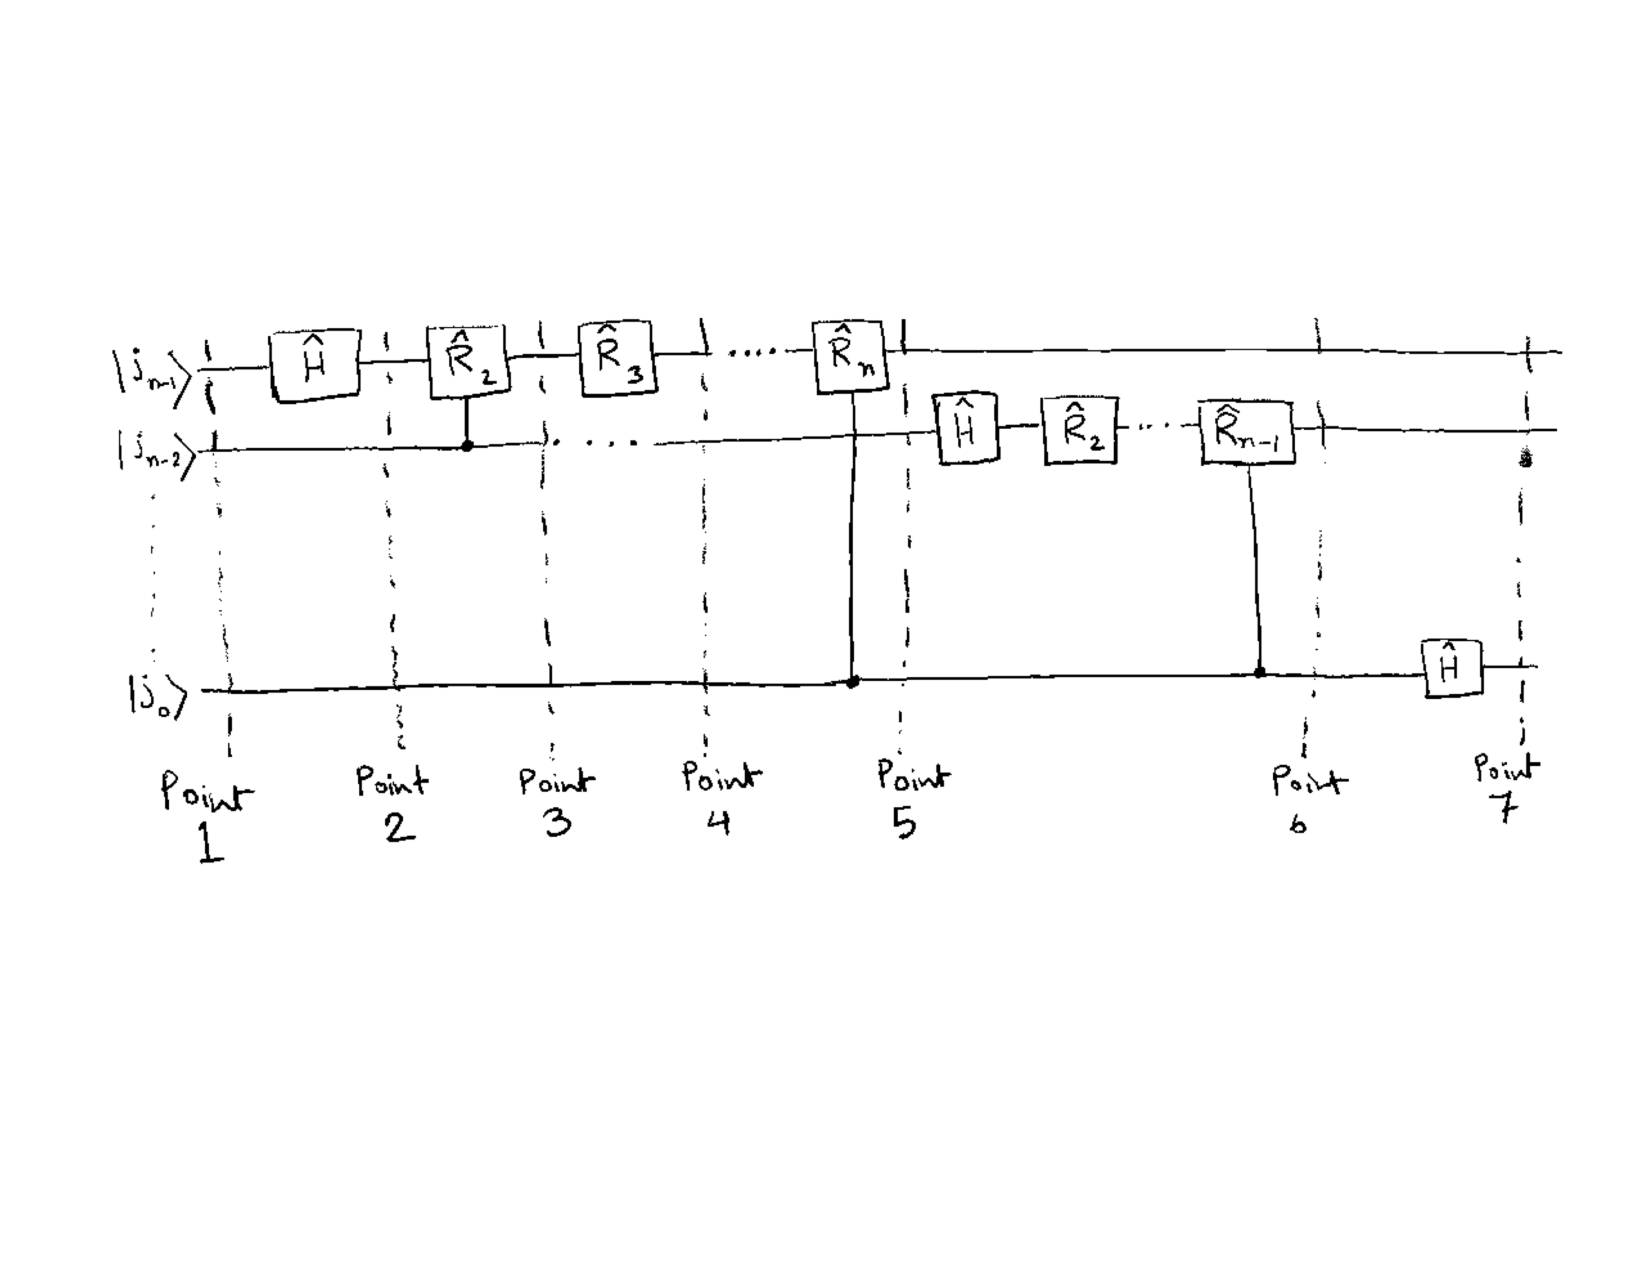
\includegraphics[width=0.99\textwidth]{QFT_diagram.pdf}
    \caption{Circuit for performing quantum Fourier transform}
    \label{QFT_circuit}
\end{figure}

\begin{enumerate}
    \item At the input point (point 1), we have the state $$\ket{j_{n-1} j_{n-2}\hdots j_1 j_0}.$$
    Remember that this is the $j$-th computational basis vector and so the qubits represent the integer $j$ in binary form.
    \item Then a Hadamard gate acts on the topmost qubit, leaving the others intact. Consequently, at point 2 we have 
    \begin{align*}
        \left(\hat{H}\ket{j_{n-1}}\right)\otimes\ket{j_{n-2}\hdots j_1 j_0} = \frac{1}{\sqrt{2}}\left(\ket{0}+e^{\frac{2\pi i j_{n-1}}{2}}\ket{1}\right)\otimes \ket{j_{n-2}\hdots j_1 j_0}
    \end{align*}
    \item Next a controlled rotation $\hat{\mathrm{CROT}}_2$ is applied on the topmost target qubit with the qubit below it serving as the control qubit. The resulting state at point 3 is
    \begin{align*}
\hat{\mathrm{CROT}}_2\left(\ket{0}\otimes\ket{j_{n-2}}+e^{\pi i j_{n-1}}\ket{1}\otimes\ket{j_{n-2}}\right)\otimes \frac{1}{\sqrt{2}}\ket{j_{n-3}\hdots j_0}
    \end{align*}
    Note from the circuit diagram that, of the two qubits involved in the $\hat{R}_2$ operation, the state $\ket{j_{n-2}}$ acts as the control qubit. Note that $$\hat{R}_2\ket{0}=e^{\frac{2\pi i.0}{2^2}}\ket{0}=\ket{0},$$
    and therefore, 
    $$\hat{\mathrm{CROT}}_2\left(\ket{0}\otimes\ket{j_{n-2}}\right) = \ket{0}\otimes\ket{j_{n-2}}.$$
    What about $\hat{\mathrm{CROT}}_2 \ket{1}\otimes\ket{j_{n-2}}$?
    If $\ket{j_{n-2}}=\ket{0}$, then obviously the state remains intact:
    \begin{align*}
        \hat{\mathrm{CROT}}_2 \ket{1}\otimes\ket{j_{n-2}} &{}= \ket{1}\otimes\ket{j_{n-2}}\\
        &{} = e^{\frac{2\pi ij_{n-2}}{2^2}}\ket{1}\otimes\ket{j_{n-2}}
    \end{align*}
    
    If $\ket{j_{n-2}}=\ket{1}$ then
    \begin{align*}
        \hat{\mathrm{CROT}}_2 \ket{1}\otimes\ket{j_{n-2}} &{} = e^{\frac{2\pi i.1}{2^2}}\ket{1}\otimes\ket{j_{n-2}}\\
        &{} = e^{\frac{2\pi ij_{n-2}}{2^2}}\ket{1}\otimes\ket{j_{n-2}}
    \end{align*}
    
    Then the state at point 3 simplifies to
    \begin{align*}
       &{} \left(\ket{0}\otimes\ket{j_{n-2}}+e^{\pi i j_{n-1}}e^{\frac{2\pi i j_{n-2}}{2^2}}\ket{1}\otimes\ket{j_{n-2}}\right) \otimes \frac{1}{\sqrt{2}}\ket{j_{n-3}\hdots j_0}\\
       &{} = \left(\ket{0}+e^{2\pi i \left(\frac{j_{n-1}}{2^1}+\frac{j_{n-2}}{2^2}\right)}\ket{1}\right) \otimes \frac{1}{\sqrt{2}}\ket{j_{n-2}\hdots j_0}\\
    \end{align*}
    \item In an identical way, it follows that the state at point 4 is
    \begin{align*}
         \left(\ket{0}+e^{2\pi i \left(\frac{j_{n-1}}{2^1}+\frac{j_{n-2}}{2^2}+\frac{j_{n-3}}{2^3}\right)}\ket{1}\right) \otimes \frac{1}{\sqrt{2}}\ket{j_{n-2}\hdots j_0}
    \end{align*}
    \item In this way, the topmost qubits picks up a phase with every controlled rotation upto point 5. At this point the state becomes
    \begin{align*}
        &{}\left(\ket{0}+e^{2\pi i \sum_{t=0}^{n-1}\frac{j_t}{2^{n-t}}}\ket{1}\right) \otimes \frac{1}{\sqrt{2}}\ket{j_{n-2}\hdots j_0}\\
        &{}=\left(\ket{0}+e^{2\pi i\frac{j}{2^n}}\ket{1}\right) \otimes \frac{1}{\sqrt{2}}\ket{j_{n-2}\hdots j_0}
    \end{align*}
    where we have used Eq.~\ref{EqBinaryExpansion}.
    From now on, the topmost qubit remains unchanged.
    \item In a similar manner, beyond point 6, the the next qubit (the one below the topmost qubit) remains unchanged. At this point, the state of the system is
    \begin{align*}
        \left(\ket{0}+e^{2\pi i\frac{j}{2^n}}\ket{1}\right) \otimes \left(\ket{0}+e^{2\pi i\frac{j}{2^{n-1}}}\ket{1}\right) \otimes \frac{1}{\sqrt{2^2}}\ket{j_{n-2}\hdots j_0}
    \end{align*}
\item Finally, at point 7, the state is
\begin{align*}
    \frac{1}{\sqrt{2^n}} \left(\ket{0}+e^{2\pi i\frac{j}{2^n}}\ket{1}\right) \otimes \left(\ket{0}+e^{2\pi i\frac{j}{2^{n-1}}}\ket{1}\right) \otimes \hdots \otimes \left(\ket{0} + e^{\frac{2\pi ij}{2}}\ket{1}\right)
\end{align*}
\end{enumerate}

\end{document}
